% Kanoon-Bridge paper draft (ACL format). Compile on Overleaf: upload this folder (acl.sty,
% acl_natbib.bst, references.bib, figures from ../../results/figures). Numbers are from the
% committed tables in results/tables; see docs/PROJECT.md for every experiment and caveat.
% Items marked \todo{} must be filled before submission.
\documentclass[11pt]{article}
\usepackage[review]{acl}            % [final] for the camera-ready version
\usepackage{times}
\usepackage{latexsym}
\usepackage[T1]{fontenc}
\usepackage[utf8]{inputenc}
\usepackage{microtype}
\usepackage{inconsolata}
\usepackage{booktabs}
\usepackage{graphicx}
\usepackage{xcolor}
\newcommand{\todo}[1]{\textcolor{red}{[TODO: #1]}}

\title{When the Law Is Renumbered: Temporal Misgrounding in Legal Retrieval\\
at India's 2024 Criminal-Code Replacement}

\author{Gaurav Rai \\
  \todo{affiliation} \\
  \texttt{gauravrai2114@gmail.com}}

\begin{document}
\maketitle

\begin{abstract}
On 1 July 2024 India replaced its three criminal codes in a single day: the Indian Penal Code
(IPC) by the Bharatiya Nyaya Sanhita (BNS), the Code of Criminal Procedure by the BNSS and the
Evidence Act by the BSA. Sections were renumbered wholesale, so the same number now names
different offences in the two codes (IPC 302 is murder; BNS 302 is not), and which code applies
depends on the date of the incident, not of the question. Legal retrieval and retrieval-augmented
generation (RAG) systems that ignore this \emph{temporally misground} their answers. We study the
problem end to end. (1) We show from 1,701 High Court criminal judgments that the transition is
slow: in 2025 only 10--29\% of judgments a month cite the BNS. (2) We measure, per provision, how
far the law moved (\emph{statutory drift}), with clause alignment, a punishment parser and
cross-code renumbering; it detects changed provisions with F1 0.89 against an independent gold
standard, where text similarity reaches 0.62. (3) We build a retrieval agent that routes questions,
verifies the code in force and the provision family of its statutes, and an answer layer that
\emph{computes} the punishment from the statute and verifies every claim. On the IL-PCSR corpus
the agent improves procedure-law retrieval from 0.859 to 0.903 MAP and Hindi/Hinglish questions
from 0.461 to 0.536 (both $p_{\text{Holm}}<0.05$); on the written facts of 995 real bail orders it
doubles MAP over the version-aware core; the answer layer states the right punishment for 86\% of
273 BNS questions where an extractive answer does for 6\%, and catches 82--100\% of injected
errors with no false alarms on clean answers. We release the system, six benchmarks, and an annotation kit, and
report our negative results: drift-aware down-ranking of old precedent, citation voting, and
table-of-contents navigation in the style of STAIR do not help.
\end{abstract}

\section{Introduction}
Legal research is a temporal task: the law that governs a case is the law in force when the facts
occurred. Most legal retrieval benchmarks ignore this because statutes change slowly, one
amendment at a time. Recent work has started to measure the failure, under the name
\emph{temporal misgrounding}: citing the version of a provision in force today when an earlier one
applies \citep{fiscalqa}, with temporal failure modes in statutory QA \citep{oldfriend} and
time-aware agentic search \citep{timetravel}.

India's 2024 replacement of its criminal codes is the extreme case of the problem. Three codes
were replaced on one day; about 500 IPC sections map to BNS sections through a many-to-many
crosswalk, and almost every number changed. A bare section number is ambiguous (``section 84'',
``section 302''); an incident in June 2024 and one in August 2024 fall under different codes; and
the precedent built on the IPC over 160 years transfers to the BNS only where the provision did
not change. Legal RAG tools still hallucinate \citep{magesh2025}; here, even a correct citation can
be correct for the wrong date.

We ask three questions. \textbf{How long do both codes stay in use?} From eCourts judgments we show
that 18 months after the switch most High Court criminal judgments still cite the IPC
(\S\ref{sec:shift}). \textbf{How far did each provision move?} We measure statutory drift per
provision and validate it against two independent gold sources (\S\ref{sec:drift}).
\textbf{Can a retrieval and RAG system be made date-correct and verifiable?} We build Kanoon-Bridge
(\S\ref{sec:system}) and evaluate it on IL-PCSR \citep{ilpcsr} and five new benchmarks
(\S\ref{sec:results}).

Our contributions: (i) evidence of a slow transition from 1,701 judgments; (ii) a statutory-drift
measure with an independent validation; (iii) a verified retrieval agent and a computed,
claim-checked answer layer, evaluated with Holm-corrected significance tests on the full IL-PCSR
corpus and on real case facts; (iv) six benchmarks (collisions, temporal penal and procedure
questions, punishment QA, facts$\rightarrow$charges, IPC-numbered questions over BNS-era
judgments) and an LLM misgrounding harness; (v) a detector of overruled precedent from the
judgments' own sentences; and (vi) negative results that bound what works.

\section{Related work}
\paragraph{Indian legal IR.} IL-TUR \citep{iltur} and IL-PCSR \citep{ilpcsr} provide prior-case and
statute retrieval benchmarks; both predate the BNS. Mapping datasets between the old and new codes
exist \citep{ieeemapping}, but we know of no retrieval or RAG evaluation of the transition.
\paragraph{Temporal and versioned legal retrieval.} Point-in-time retrieval over versioned
norms \citep{satgraph,frbr}, temporal statutory QA \citep{oldfriend,timetravel} and temporal
misgrounding \citep{fiscalqa} study gradual amendment. We study a one-day, three-code
replacement with colliding numbers, where version selection alone is not enough: the right
section of the new code must also be found.
\paragraph{Verified RAG.} Citation support is evaluated by ALCE \citep{alce}; corrective RAG
\citep{crag} repairs retrieval; adaptive RAG \citep{adaptiverag} routes by question type; legal
hallucination benchmarks check citations claim by claim \citep{lephantomcite,parcel}. Our answer
layer computes what can be computed (punishments) instead of generating it, and checks numbers,
sections, code in force, negation and quotations.
\paragraph{Structure-aware retrieval and KV reuse.} STAIR \citep{stair} retrieves through a
corpus's table of contents with a trained generative retriever; we test the training-free version
on statutes. RAGCache \citep{ragcache}, CacheBlend \citep{cacheblend} and tiered KV management
\citep{pactkv} reuse the KV cache of retrieved documents; we measure the reuse in legal RAG traffic.

\section{The transition in the courts}\label{sec:shift}
We sampled criminal judgments of five High Courts (Delhi, Allahabad, Punjab and Haryana, Gujarat,
Kerala) from the eCourts open dataset (CC-BY-4.0), 2023--2025, 12--30 per court and month, 1,701
in total, and extracted every section citation with a code-aware tokenizer. No judgment in the
sample cites the BNS before October 2024. Through 2025, 10--29\% of judgments per month cite the
BNS and 25--35\% still cite the IPC (Figure~\ref{fig:shift}): most pending cases concern
incidents before 1 July 2024, so both codes will be cited for years.

\begin{figure}[t]
\centering
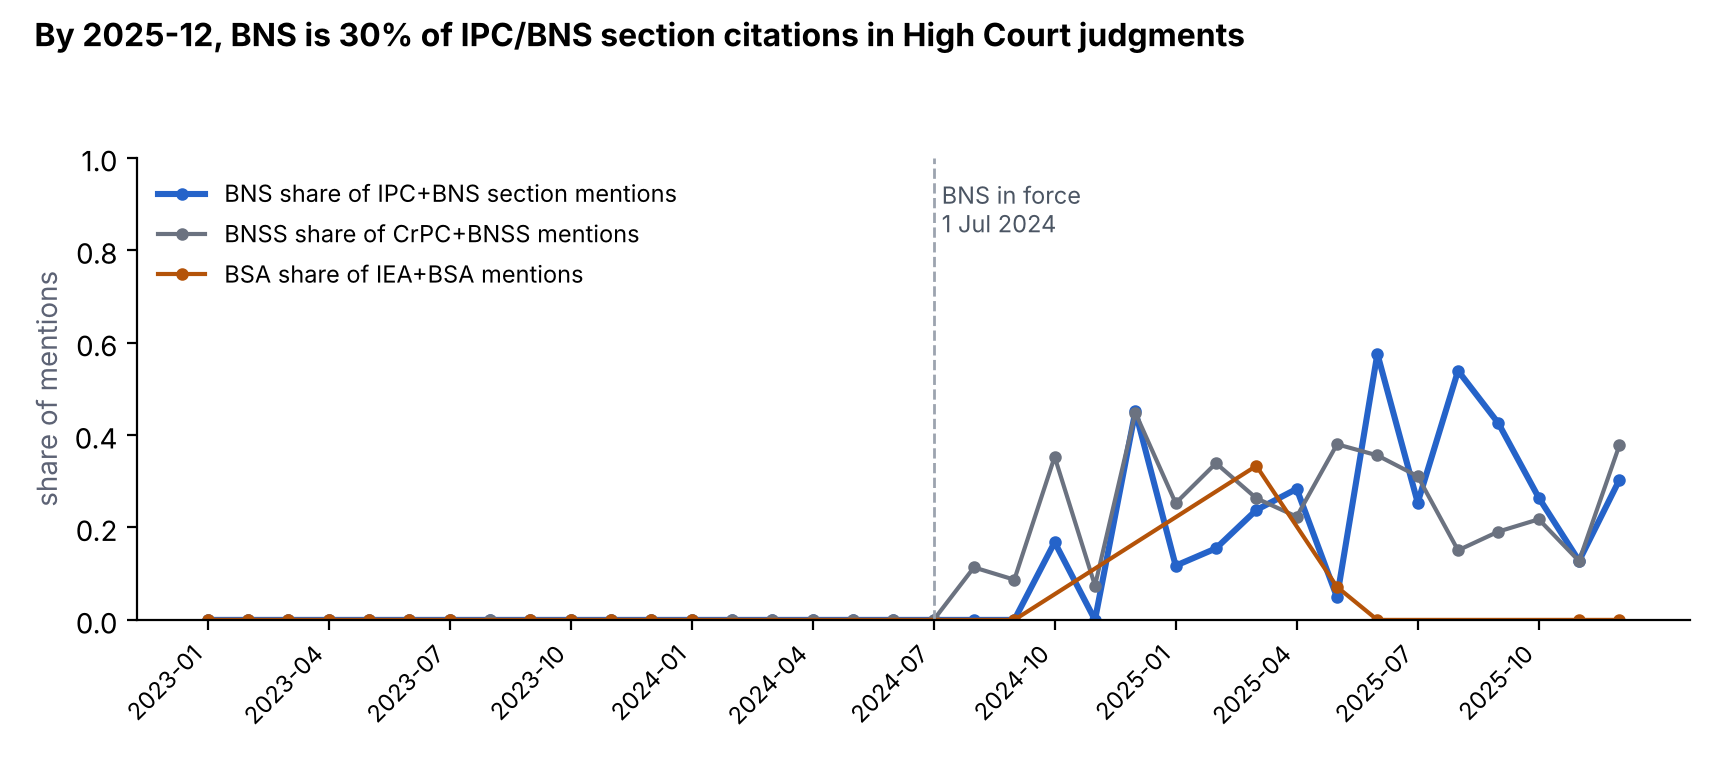
\includegraphics[width=\columnwidth]{figures/citation_shift.png}
\caption{Share of High Court criminal judgments citing the IPC and the BNS, per month (eCourts,
1,701 judgments).}
\label{fig:shift}
\end{figure}

\section{Statutory drift}\label{sec:drift}
For every new-code section and its predecessor(s) we compute a drift vector: clause-level
retention and novelty by word-bigram containment \citep{broder1997} after rewriting cross-references
into the new numbering; a parsed punishment structure (death, life, minimum and maximum terms,
fine caps, community service, number words); mental-state words and quantified thresholds; and
merge/split structure. Hand-set rules map it to classes (identical, cosmetic, restructured,
punishment, substantive, new, repealed) and to a pairwise \emph{carry-over} score: how much of the
old provision's precedent applies to the new one. The text is India Code's consolidated text
(kanoonhq/open-laws, CC0).

\paragraph{Validation.} Two independent gold sources label the 346 BNS sections with an IPC
predecessor: S1, a section-level retained/changed mapping, and S2, change notes we read with rules;
they agree at $\kappa=0.75$. On a held-out half (Table~\ref{tab:drift}), the drift vector with a
logistic regression reaches F1 0.89 on S1 and 0.81 on S2; the best text-similarity baseline 0.62
and 0.68; the official crosswalk's own relation 0.21 and 0.32 (McNemar $p<0.001$). Punishment
parsing carries most of the signal: most BNS changes are raised fines and terms, one-word edits that
similarity cannot see. Repeal detection reaches AUC 0.96. For the CrPC$\rightarrow$BNSS and
Evidence Act$\rightarrow$BSA families, plain edit similarity is as good (0.78 vs 0.75; 0.53 vs
0.40): a negative result outside penal law.

\begin{table}[t]
\centering\small
\begin{tabular}{lcc}
\toprule
System & F1 (S1) & F1 (S2) \\
\midrule
Crosswalk relation $\neq$ ``same'' & 0.21 & 0.32 \\
Edit similarity (tuned on dev) & 0.62 & 0.68 \\
Drift rules (hand-set) & 0.85 & 0.76 \\
Drift vector + logistic regression & \textbf{0.89} & \textbf{0.81} \\
\bottomrule
\end{tabular}
\caption{Which IPC provisions changed in the BNS (held-out half, 183 sections).}
\label{tab:drift}
\end{table}

\section{System}\label{sec:system}
\paragraph{Version-aware core.} IPC and BNS sections (and CrPC/BNSS, IEA/BSA provisions) share
offence ids through the crosswalk, in the index, the query analyzer, Boolean search and the
statute-to-precedent bridge; statutes are filtered to the code in force on the incident date;
bare colliding numbers are resolved from context. Ranking is BM25F over judgment zones with
citation-graph authority, a word-trigram channel and a learned re-ranker; spelling correction,
transliteration and a Hinglish legal lexicon handle typed queries.
\paragraph{Agent.} The agent routes a question (pasted judgment / section lookup / fact question),
chooses the code family (penal, procedure, evidence) from the statutes and precedents it
retrieved, runs a family-restricted statute search, and \emph{verifies} its top statutes: family,
code in force, stemmed heading specificity against the spelling-corrected question, and a penalty
for definition sections. Fact questions are decomposed into the chosen statute's sub-sections,
whose evidence coverage is reported in a research memo.
\paragraph{Answer layer.} The structured answer names the provision in force, \emph{computes} its
punishment per sub-section with the drift punishment parser, and quotes one precedent sentence.
Every sentence of an answer (structured or generated) is verified against its cited source: idf
support or, for a stated punishment, structural agreement with the statute's parsed punishment;
every quantity must appear in the source; every section must be the source's own, cited by it, or
its counterpart; the code must be in force; a negation the source lacks is a contradiction;
quotations must be verbatim. Failing sentences are regenerated once with the problems listed (LLM)
and then repaired: old-code sections swapped to their counterparts, contradicted sentences replaced
by the source's words, unsupported ones removed, each action shown to the user.
\paragraph{Judicial treatment.} Precedent can also be made stale by a court. We extract
treatment (overruled, per incuriam, doubted, followed) from the judgments' own sentences,
attach it to the case it governs with rules against misattribution (``\emph{in view of} X'',
``\emph{in} X \emph{this Court overruled} Y'', negation), and link case names to the corpus by
party names. Overruled judgments are down-ranked and explained.

\section{Experiments}\label{sec:results}
\paragraph{Data.} IL-PCSR \citep{ilpcsr}: 3,183 precedents, 936 statutes, 627 test queries; plus
the BNS, BNSS and BSA. Benchmarks: E2 colliding numbers (252), E4 Hindi/Hinglish/English needs with
two judges (50), E6 jurisdiction (40), E7 penal provisions before/after 1 July 2024 (200), E9
procedure and evidence (342), E14 punishment QA (273 BNS sections, gold from an independent
summary), E19 facts$\rightarrow$charges (995 bail orders of IndianBailJudgments-1200
\citep{bail1200}, first 60 words of the facts, scored code-blind), E10 IPC-numbered questions over
BNS-era judgments (39 questions, 348 judgments). Significance: paired randomization tests on
per-query AP, Holm-corrected over all comparisons \citep{smucker2007}.

\paragraph{Retrieval (Table~\ref{tab:retrieval}).} The agent improves the questions about the
law: procedure (+0.044 MAP, $p_{\text{Holm}}=0.04$), Hindi/Hinglish (+0.075, $p_{\text{Holm}}=0.04$)
and penal (+0.035; 28 wins, 8 losses). Removing the verifier undoes the gains (E7 0.873, E9 0.845).
On whole judgments as queries (E1) it keeps the core ranking (1.1 searches per query), where a
rule-planner agent lost 0.11 MAP. On E6 both agents trade MAP for the top of the list (P@1 0.80
$\rightarrow$ 0.90, all top-5 results binding). On real case facts (E19) it doubles the core's MAP
(0.047 $\rightarrow$ 0.100) and nearly triples hit@1 (0.06 $\rightarrow$ 0.17) \todo{paired test
from results/tables/facts\_ilpcsr\_significance.csv}. On E10, the shared offence ids let IPC-numbered
questions find BNS-era judgments (MAP 0.004 for BM25 $\rightarrow$ 0.151; 32 wins, 2 losses,
$p<0.001$).

\begin{table}[t]
\centering\small
\begin{tabular}{lccc}
\toprule
Set (MAP) & core & agent v1 & agent v2 \\
\midrule
E1 judgments$\rightarrow$precedents & \textbf{.414} & .306 & .412 \\
E2 colliding numbers & .885 & \textbf{.936} & .921 \\
E4 Hindi / Hinglish & .461 & .460 & \textbf{.536}$^\dagger$ \\
E6 jurisdiction & \textbf{.630} & .554 & .554 \\
E7 penal, by date & .880 & .877 & \textbf{.915} \\
E9 procedure, by date & .859 & .859 & \textbf{.903}$^\dagger$ \\
E19 bail facts$\rightarrow$charges & .047 & .057 & \textbf{.100} \\
\bottomrule
\end{tabular}
\caption{Retrieval on the IL-PCSR corpus. $^\dagger$ $p_{\text{Holm}}<0.05$ vs core.}
\label{tab:retrieval}
\end{table}

\paragraph{Answers (Table~\ref{tab:answers}).} An extractive answer quotes the statute's best
sentence, which is rarely its punishment clause (6\% right); the computed answer states the right
punishment for 86\% of questions, 93\% when the statute is right. In error injection, the claim
verifier flags a changed term in 89\% of answers (cosine support: 30\%), a flipped negation in 83\%
(30\%), a wrong section in 100\% (34\%) and another statute's punishment in 89\% (36\%), with no
false alarm on clean answers (84\% for cosine support). Injection uses the error types the verifier
was designed for, so these rates are upper bounds.

\begin{table}[t]
\centering\small
\begin{tabular}{lcc}
\toprule
System & statute@1 & punishment right \\
\midrule
core + extractive answer & .912 & .062 \\
core + computed, verified answer & .912 & .854 \\
agent + computed, verified answer & \textbf{.927} & \textbf{.861} \\
\bottomrule
\end{tabular}
\caption{Punishment QA on the IL-PCSR corpus (273 BNS questions, incident date 2025).}
\label{tab:answers}
\end{table}

\paragraph{LLM misgrounding.} \todo{E20: run scripts/19\_eval\_misgrounding.py with an open 7--8B
model (and one API model) under closed-book, naive RAG, date-aware RAG, verified RAG; report
right@1, misgrounded@1 and any-wrong-code per set. This is the paper's central LLM result.}

\paragraph{Judicial treatment.} From the precedent pool and training queries, the extractor finds
5 overruled judgments (Golak Nath, United Motors, Northern India Caterers, Air India Statutory
Corporation, Balsara in part), all correct on our check \todo{confirm with the annotation round};
an unconstrained attachment found 10, half wrong. Recall is low, and in E1 flagged judgments reach
the top 10 for only 0.6\% of queries: a safety signal, not a ranking gain.

\section{Negative results}
\paragraph{Down-ranking stale precedent.} Penalising old-code precedents by (1$-$carry-over) leaves
unchanged provisions untouched but costs citation-MAP on substantively changed ones (0.32
$\rightarrow$ 0.22) without reducing stale results in the top 10, which are rare (at most 1.5\%).
Citation relevance counts stale precedent as relevant; the signal is better shown than ranked.
\paragraph{Citation voting.} Statutes voted for by the retrieved precedents help with eight
synthetic precedents and hurt with real ones: with 1,701 real judgments they promote the most cited
sections and cost 0.15 on colliding-number questions.
\paragraph{Table-of-contents navigation.} Choosing chapters by their table-of-contents entries
(chapter, Gazette sub-heading, section headings), as STAIR does with a trained retriever, did not
help without training: flat on E7 and E19, worse on E2 (0.857 $\rightarrow$ 0.762) and E9 (0.877
$\rightarrow$ 0.854). Chapter names are too coarse to choose between neighbouring sections.
\paragraph{KV reuse.} In a trace of 2,082 legal RAG questions, 63\% of prompt tokens repeat an
earlier question's chunk (78\% for statutes), but the working set is large (about 80\,GiB of
Mistral-7B KV): a 4\,GiB cache serves 19\% of tokens with LFU and 10\% with LRU. Frequency beats
recency, as tiered KV managers argue \citep{pactkv}; the gain needs tiering, not a larger cache.

\section{Conclusion}
A code replacement turns legal retrieval into a temporal problem with colliding identifiers.
Date-aware statute selection, verified answers and computed punishments make a measurable
difference; down-ranking old precedent does not. The transition will last years, and the
benchmarks and system we release make it measurable.

\section*{Limitations}
No LLM has yet been evaluated (E20). Two fixes were found by looking at test results (statute
headings read from the text for IL-PCSR's bare titles; structural punishment support) and are
declared in the release; E19 was run after them and was not used to decide them. The drift gold
labels are section-level and one of them is our rule-based reading of notes; human labels are
being collected with the released kit. E7, E9 and E14 questions are phrased like section headings;
E4 and E19 are not. The treatment detector's recall is low.

\section*{Ethics statement}
The system is a research tool, not legal advice; answers show their sources and corrections. All
data are public court judgments and legislation under their licences (IL-PCSR CC-BY-NC-SA,
eCourts CC-BY-4.0, India Code CC0, IndianBailJudgments-1200 CC-BY-4.0); raw data are not
redistributed.

\bibliography{references}

\end{document}
